\documentclass[10pt]{beamer}
\usepackage[english]{babel}


\usepackage{subfig}

\title{Cooling Loop}
\author{Anja Beck}
\date{\today}
\institute{DESY Hamburg}


\definecolor{craneorange}{rgb}{0.68,1,1}
\setbeamertemplate{blocks}[rounded][shadow=false]
\setbeamertemplate{footline}[page number]
\beamertemplatenavigationsymbolsempty 
\usepackage{pgfpages}
%\setbeameroption{show notes}
%\setbeameroption{show notes on second screen=right}

%\usetheme{Hannover}
\usecolortheme{crane}

\usepackage[
	separate-uncertainty=true,
	per-mode=symbol-or-fraction,
]{siunitx}

\begin{document}
	%	\setbeamertemplate{frametitle}[default][center]
	
	\begin{frame}[plain,noframenumbering]
		\titlepage
	\end{frame}
\begin{frame}{RI Images Cooling Loop}
	\begin{figure}
		\centering
		\includegraphics[width=0.24\textwidth]{../Labels/LabelsLeft.pdf}
		\includegraphics[width=0.24\textwidth]{../Labels/LabelsCentreLeft.pdf}
		\includegraphics[width=0.24\textwidth]{../Labels/LabelsCentreRight.pdf}
		\includegraphics[width=0.24\textwidth]{../Labels/LabelsRight.pdf}
	\end{figure}
\end{frame}
\begin{frame}{Left}
	\begin{figure}
		\centering
		\includegraphics[width=0.9\textwidth]{../Labels/LabelsLeft.pdf}
	\end{figure}
\end{frame}
\begin{frame}{CentreLeft}
	\begin{figure}
		\centering
		\includegraphics[width=0.9\textwidth]{../Labels/LabelsCentreLeft.pdf}
	\end{figure}
Note: I saved this image too early. There are ten labels, enumerated 41-50, missing. They are situated at the vertical lower pipe.
\end{frame}
\begin{frame}{CentreRight}
	\begin{figure}
		\centering
		\includegraphics[width=0.9\textwidth]{../Labels/LabelsCentreRight.pdf}
	\end{figure}
\end{frame}
\begin{frame}{Right}
	\begin{figure}
		\centering
		\includegraphics[width=0.9\textwidth]{../Labels/LabelsRight.pdf}
	\end{figure}
\end{frame}
\begin{frame}{Which labels were used?}
	\begin{figure}
		\centering
		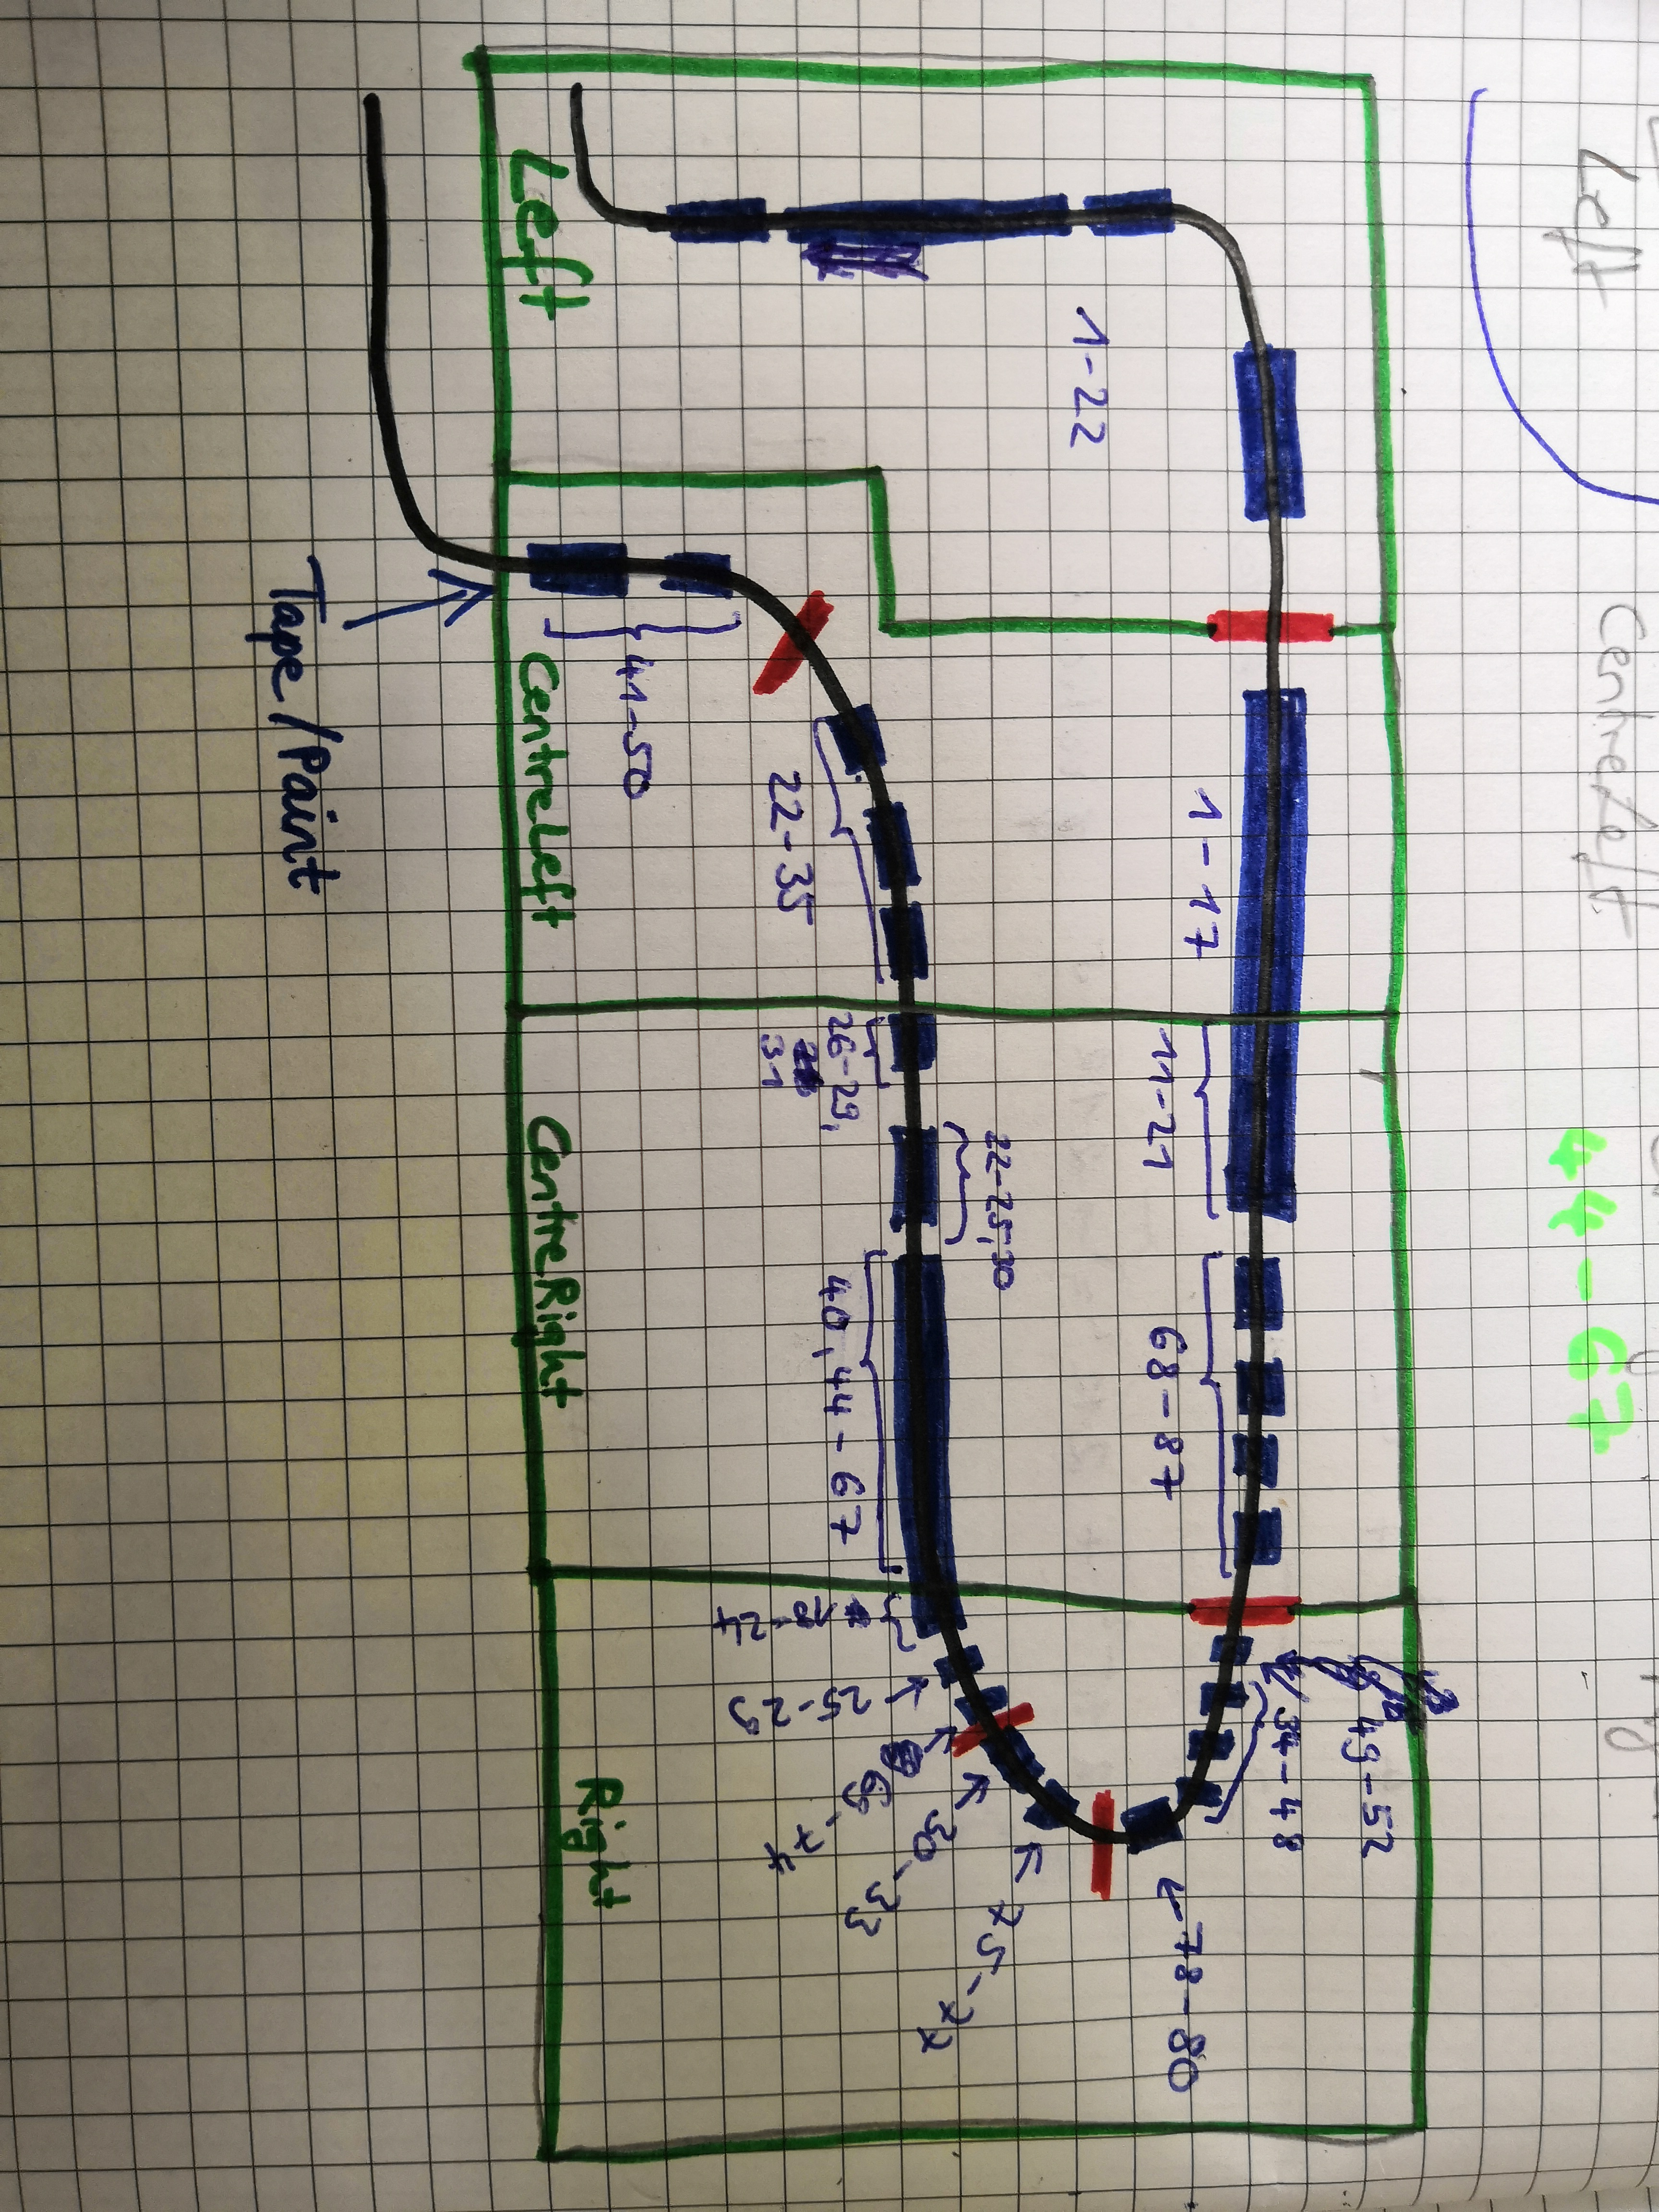
\includegraphics[width=0.75\textwidth, angle=90,origin=c]{../Labels/Schematics.jpg}
	\end{figure}
\end{frame}
\begin{frame}{Temperatures}
	\begin{figure}
		\centering
		\includegraphics[width=\textwidth]{../test.pdf}
	\end{figure}
	From left to right, those are the measurement points starting at the upper pipe entry and ending at the lower pipe entry. The labels state T/B for top or bottom pipe, then the picture to which they refer, and the number of the label itself.
\end{frame}
\end{document}